\documentclass[10pt]{article}
\usepackage[utf8]{inputenc}
\usepackage[spanish]{babel}
\usepackage{amsmath}
\usepackage{amsfonts}
\usepackage{amssymb}
\usepackage{graphics}
\usepackage{graphicx}
\usepackage[left=2cm,right=2cm,top=2cm,bottom=2cm]{geometry}
\usepackage{imakeidx}
\makeindex[columns=3, title=Alphabetical Index, intoc]
\usepackage{listings}
\usepackage{xcolor}
\usepackage{multicol}
\usepackage{changepage}
\usepackage{float}
\usepackage{cite}
\usepackage{url}
\usepackage{hyperref}
\usepackage[document]{ragged2e}
\hypersetup{
    colorlinks=true,
    linkcolor=blue,
    filecolor=magenta,
    urlcolor=blue,
}

\definecolor{codegreen}{rgb}{0,0.6,0}
\definecolor{codegray}{rgb}{0.5,0.5,0.5}
\definecolor{codepurple}{rgb}{0.58,0,0.82}
\definecolor{backcolour}{rgb}{0.95,0.95,0.92}

\lstdefinestyle{mystyle}{
    backgroundcolor=\color{backcolour},
    commentstyle=\color{codegreen},
    keywordstyle=\color{magenta},
    numberstyle=\tiny\color{codegray},
    stringstyle=\color{codepurple},
    basicstyle=\ttfamily\footnotesize,
    breakatwhitespace=false,
    breaklines=true,
    captionpos=b,
    keepspaces=true,
    numbers=left,
    numbersep=5pt,
    showspaces=false,
    showstringspaces=false,
    showtabs=false,
    tabsize=3
}

\lstset{style=mystyle}

\title{Actividad No. 4 Correción\\ Solución de problemas mediante Ascensión de Colinas\\Laboratorio 1}

\author{Adrian González Pardo}

\date{\today}

\newcommand\tab[1][1cm]{\hspace*{#1}}

\begin{document}
\maketitle
\section{Ventajas y desventajas de la Ascensión de Colinas}
Inicialmente el espacio de soluciones de un problema puede ser representado en una grafíca en $R^{2}$, $R^{3}$, hasta $R^{n}$ por lo que podemos explorar su espacio mediante una heuristica la cual es generalmente el Ascensio de Colinas el cual proporciona las siguientes ventajas y desventajas:
\begin{center}
  \begin{tabular}{| p{6cm} | p{6cm} | }
    \hline
    Ventajas & Desventajas
    \\\hline
    Permite realizar un número menor de iteraciones con respecto a la exploración del espacio en modalidad de fuerza bruta & El resultado puede quedarse en un minimo local sin que sea el minimo del espacio\\
    \hline
    Permite moverse en el espacio de diferentes formas, permitiendo que encuentre un minimo & Dependiendo de la implementación del algoritmo puede que que llegue al minimo o no, pero al final arroja una solución\\\hline
    Dependiendo de la implementación puede que tenga un número distinto de iteraciones & En caso de ser un espacio muy grande puede que la implementación, salto o movimiento entre el espacio demore demasiado\\\hline
  \end{tabular}
\end{center}
\section{Pseudocódigo del Algoritmo Steepest Ascent Hill Climbing (Ascenso Más Empinado Escalada de Colinas)(SAHC)}
\lstinputlisting[language=C]{sahc.c}
\section{Next-Ascent Hill-Climbing (Próxima Ascenso Escalado)(NAHC)}
\lstinputlisting[language=C]{nahc.c}
\section{Random-Mutation Hill-Climbing (Ascenso Por Mutación Aleatoria)(RMHC)}
\lstinputlisting[language=C]{rmhc.c}
\section{Resultados de Forrest y Mitchell}
Si bien en sus conclusiones nos podemos dar cuenta en cuestios de los algoritmos heuristicos SAHC y NAHC en la busqueda de soluciones de un espacio bidimensional no encontraron la zona optima, el algoritmo RMHC lo encontro en un número menor de iteraciones con respecto a los algoritmos geneticos que se implementaron en la investigación, esto pasa en relación a que el algoritmo RMHC explora el espacio de soluciones en este caso digamos o aproximemos en grafos es más sencillo tomar la decisión sobre que nodo iterar sin realizar tantas comparaciones.
\section{Aplicaciones de Algoritmos de Ascenso de Colinas}
Si bien en muchas ocasiones estos algoritmos se ven como una caja negra a la hora de ser utilizados en muchos modulos o toolbox de lenguajes de programación estos estan intimamente aplicados en el cálculo de gradiente descendente de $N$ variables para optimizar un aprendizaje supervisado o no supervisado, donde sobre cada iteración se realiza el calculo de un nuevo movimiento en el espacio de soluciones, por otro lado tambien este tipo de algoritmo esta implementado en algunas aplicaciones en las que se realiza la planificación de rutas de transporte e incluso en sistemas de reconocimiento de objetos 3D, una vez más retomando los terminos del Aprendizaje de Maquina podemos encontrar desde regresión lineal, polinomial y logistica.
\section{Aplicación de RMHC en distintos problemas con su estructura de datos}
\subsection{Knapsack Problem}
\[f(x)=\sum_{i=1}^{N}h\left(g\left(x_{i}\right)\right)\]
Donde:
\[x_{i}\;\;es\;un\;objeto\;que\;puede\;almacenarse\;en\;la\;mochila\]
\[g(x)\;\;es\;una\;funcion\;booleana\;la\;cual\;nos\;dice\;si\;x_{i}\;esta\;en\;la\;solucion\]
\[h(x)\;\;es\;una\;funcion\;la\;cual\;devuelve\;el\;valor\;de\;beneficio\;por\;el\;objeto\;x_{i}\]
De esta forma igual se cubre una segunda función la cual es:
\[p(x)=\sum_{i=1}^{N}m\left(g(x_{i})\right)\;<=\;Peso\_maximo\]
Donde:
\[m(x)\;\;es\;una\;funcion\;la\;cual\;devuelve\;el\;peso\;que\;a\tilde{n}ade\;a\;la\;mochila\;por\;cada\;objeto\;x_{i}\]
De tal forma que la suma de pesos para resolver este problema debe de ser menor igual al peso máximo que tiene la mochila de capacidad.\\
Los estados iniciales de este problema son:
\begin{itemize}
  \item El conjunto de objetos que pueden pertenecer a la mochila
  \item Una solución inicial la cual es valida para el peso maximo de la solucion
  \item Segun el algoritmo de RMHC el best\_solution y new\_best es una cadena de bits las cuales si estan en 1 significara que el objeto en la mochila de acuerdo a la posición de cada 1 y 0
  \item f\_best y f\_new son los valores de beneficio que pueden ser agregados a la nueva solucion de acuerdo a la modificación de objetos en el paso de mutación.
\end{itemize}

En el diseño de la solución se solicita los siguientes datos:
\begin{itemize}
  \item Peso máximo de la mochila
  \item Limite de iteraciones
  \item Indice de la configuración del archivo el cual contiene la estructura de (peso,beneficio)
\end{itemize}
\textit{Ejemplo:}
\begin{center}
  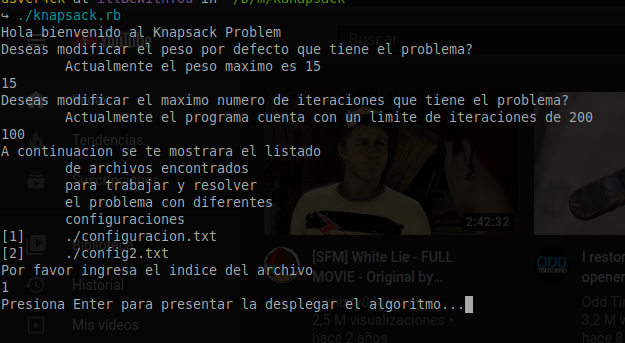
\includegraphics[scale=0.5]{imgsRMCH/knapsack.png}\\
  \textit{Figura 1 Primera parte del programa}\\
  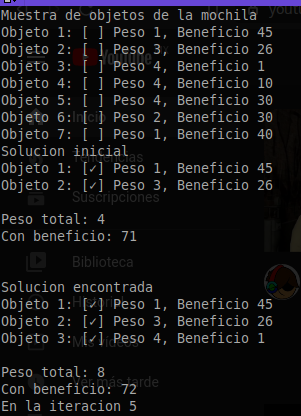
\includegraphics[scale=0.5]{imgsRMCH/knapsack1.png}\\
  \textit{Figura 2 Parte de la ejecución a partir de la implementación}
\end{center}

\subsection{Travel Salesman Problem}
La función que buscamos es la minimización de costo total del problema representado como:
\[f(x)=\sum_{i=1}^{N}g\left(h\left(x_{i}\right)\right)\]
Donde:
\[x_{i}\;\;es\;una\;arista\;de\;un\;vertice\;v_{j}\;que\;va\;a\;v_{k}\]
\[h(x)\;\;es\;una\;funcion\;que\;considera\;o\;no\;el\;trayecto\;v_{j}\;a\;v_{k}\;de\;x_{i}\]
\[g(x)\;\;es\;una\;funcion\;que\;devuelve\;el\;valor\;de\;costo\;de\;x_{i}\]
Los estados de este problema son los siguientes:
\begin{itemize}
  \item Una solución random valida de recorrido $v_{i}$ hasta $v_{j}$ de tal forma que entre desos dos existen al menos N vertices que sumados en sus costos nos dan una respuesta.
  \item Limite de iteraciones
  \item Indice de la configuración de formato ($vertice_{i}$ , $costo$ , $vertice_{j}$)
\end{itemize}
\subsection{Obtención de minimos de la función f(x)}
Función:
\[f(x)=\sum_{i=1}^{D}x_{i}^2\;\;\;\;con\;\;\;\;x_{i}\in[-10,10]\]
Para el calculo de minimos es necesario buscar inicialmente una solución random de $M$ puntos en los cuales no se garantiza que en algun $x_{i}$ sea igual a cero, por lo que es necesario apartir de esta respuesta se puede comenzar a modificar para que exista un valor aproximado de $M$ puntos minimos de acuerdo al maximo numero de iteraciones.\\
Los estados de este problema son:
\begin{itemize}
  \item Solución random de puntos $(x_{1},x_{2},\cdots,x_{D})$ de tal forma en que no todos los puntos son minimos, por lo cual consideraremos un mínimo de la función cuando algún $x_{i}=0$.
  \item Limite de iteraciones
  \item Lista de puntos a la solución random
\end{itemize}
$I_{Im}$ = ​${{g}}{Im}u^{5}z(V - E{Im})$
\end{document}
